\documentclass[12pt]{article}
% https://drive.google.com/file/d/1wRYAsCDTtx3jic7XitKq7dlXOOMHYdyj/view?usp=sharing
\usepackage{graphicx,amssymb, amstext, amsmath, epstopdf, booktabs, verbatim, gensymb, geometry, appendix, natbib, lmodern}
\geometry{letterpaper}
%\usepackage{garamond}
\usepackage{amsmath}
\usepackage{graphicx}
\usepackage[colorinlistoftodos]{todonotes}
\usepackage{float}
\usepackage{subfig}
\usepackage{lscape}
\usepackage{graphicx}
\usepackage[colorlinks,citecolor=red,urlcolor=blue,bookmarks=false,hypertexnames=true]{hyperref} 


\newcommand*\Title{Bikes}
\newcommand*\cpiType{Team 12}
\newcommand*\Date{\today}
\title{On the Adoption of Bikeshare in NYC}
\author{Team 12: Li, Lian, Pu, Stamell}
\date{\today}
%-----------------------------------------------------------

\usepackage{cpistuff/cpi} % This is what makes your document look like a cpi document.


\begin{document}

\begin{titlepage}
\maketitle
\end{titlepage}

\linespread{1.15} %Set standard document linespacing
\section*{Topic Question}
In the past 10 years, options for short-distance transportation have proliferated, including rideshare, bikeshare, and more recently scootershare models. In this report we focus on the primary question: What are the forces that impact how people commute to work? In particular, what pushes commuters to adopt Bikeshare services in New York City?

\par To understand this question, we must first ask, why would someone consider using bikeshare for their commute?\\
$\bullet$ \textbf{Convenience:} Most residents of NYC live too far from work to walk, therefore they need to some form of transportation to reach their jobs. Currently, a one-year citi bike membership costs the same as a one-month unlimited metro card.\\
$\bullet$ \textbf{Price:} Bikeshare memberships are the most affordable form of transportation in NYC. \\
$\bullet$ \textbf{Openness:} People must be willing to bike to work. New York City can be a dangerous place to bike, and some people might not want to take that risk\\


\par With this in mind, we study the extent to which bikeshare ridership affected by competing modes of services, climate and weather, socioeconomics, and the presence of bike lanes. We comment on policy recommendations for improving the viability of bikeshare in NYC.
\section*{Summary}
We study the forces that drive users to use bikeshare services in NYC, focussing on spatial and temporal dimensions. Since its introduction in 2013, Bikeshare usage has grown by more than 3-fold. What accounts for the increase of bikeshare usage? To what extent has this effected other transportation modes? We use both spatial and temporal analysis to tackle these questions. Below are our key results

$\bullet$ Effect of seasonality: We find that there is a strong seasonal dependence for bikeshare usage, but not other transportation modes (taxi, uber, subway). We find that this dependence is not directly due to the outside temperature, but rather strongly predicted by wind, rain and snow: for each 1 mph increase in wind speed, the bike ridership decreased by 2\%. For each inch of rain, the ridership decreased by 20\%, and for each inch of snow, the ridership decreased by a whopping 43\%.

In cases of bad weather, which modes saw the most gain? We found that by far, Uber ridership had the most significant correlation between with weather, at above 4-sigma levels. Every inch of rain increased Uber usage by $15\%$, and each inch of snow in fact increased Uber ridership by a whopping $700\%$. 

$\bullet$ Effect on other modes: We find that, past ridership growth in subway usage and uber and lyft rides tend to reduce future growth in bikeshare usage at statistically significant levels; whereas past ridership growth in taxis is predictive of growth in bikeshare usage.

What are the impact of increased bikeshare ridership on other transport modes? We found that bike usage decreases subway, uber and taxi ridership at statistically significant levels, with the correlation being of roughly equal strength. This shows that bikeshare is essentially replacing other modes of transport when it increases in usage. In other words, when people give up their bikes, they also tend to migrate to taxis, uber and subways in equal proportions.

\newpage
$\bullet$ Socioeconomics: we find three variables that are significant for the data set at 90\% confidence level (see table below)
\par Number of citi bike stations is the most significant variable, with a coefficient of $0.09$. For an NTA neighborhood of $\sim 50K$, this equates to a $\sim 4.5K$ increase in bike rides (per year). We also see a negative relationship between median age and rides. Unsurprisingly, as people age, it becomes more difficult to take advantage of citi bikes. Therefore, when considering where to add stations, it would be better to focus on areas with younger demographics.

$\bullet$ Presence of bike lanes: We also find that there is no statistically significant dependence between bike lane length and bike share usage, when all other variables are accounted for.

\section*{Policy Recommendations}
$\bullet$ We find that while snow by far is the biggest deterrent of bikeshare usage, riders are generally not affected otherwise by low temperatures. Aggressive snow-clearing would help increase bike ridership.

$\bullet$ We find that subway usage is not correlated with increased bike share usage. This is discouraging, since most riders are annual members and there is no marginal cost to using bike alongside subway. Since bikeshare has a role to play in solving the last-mile problem, riders should be encouraged to use bikes and subway in tandem. We suggest the reason for the lack of synergy is due to lack of fare integration: policy makers should explore providing discount or free transfers to subway for one-time bikeshare passes, or vice versa (providing free bike passes for each subway ticket).



\newpage 

\section*{Data Manipulation}
This data-set contains a very large amount of data which is infeasible to work with directly. The first take is to break this data down into more manageable proportions. In this report we focus on temporal and spatial patterns, and therefore we work towards obtaining two main datasets:

$\bullet$ 1. We obtain, for each NTA code, the total number of rides over the weekday AM and PM rush hour, for each of the following modes: bikeshare, taxis, uber/lyft, subway, over the time period of ... \\ 
$\bullet$ 2. We obtain, for the entire NYC city as a whole, the total number of rides per day for each of the following modes: bikeshare, taxis, uber/lyft, and subway. \\

In this study, we focus on the behavior of commuters specifically, because they comprise of most of the ridership, place the greatest burder on the transport system, act in predictable patterns. Moreover, since different modes cater to different purposes (e.g. tourism, commuting, city-to-airport), focussing on commuters facilitate the cross-mode comparison. In order to select for commuters, we cut the data into AM and PM rush hour (6-9 am and 3-7pm respectively) and select only the weekday data. 

We choose to look at four variables in the weather file. They are Daily Average WetBulb Temperature,Daily Average Wind Speed,	Daily Precipitation, Daily Snowfall. These four variables allow us to explore the impact of weather on people's choices of different transportation. Instead of using temperature directly, we use the difference between daily temperature and the average temperature, which is 54 F.

\newpage

$\bullet$ {\bf Distance Calculation}:\\
In this problem we are often given longitude and latitude. The distance between a pair of points in longitude-latitude assuming the Earth is flat (a reasonable assumption over the scale of NYC) can be estimated as:
\begin{equation}
\label{eq:dist}
    D \simeq R_E  \times \frac{2\pi}{360} \sqrt{\cos^2{\theta_{NYC}} (\phi_i - \phi_f)^2 + (\theta_i - \theta_f)^2},
\end{equation}
where $\phi_i, ~\phi_f, ~\theta_i, ~\theta_f$ are the initial longitude, final longitude, initial latitude and final latitudes respectively in degrees, $\theta_{NYC} \approx 40.5$ deg. is the approximate latitude of NYC, and $R_E \simeq 6378$ km is the radius of the Earth. 


\section*{Additional Datasets}
In addition to data provided, we also made use of external data-sets, relating to the GIS coordinates of NYC NTA area codes, as well as the distribution and length of the bike lanes network.

$\bullet$ NYC bike lanes data: We downloaded the GIS geo-spatial bike lanes data (as of 2017) from NYC OpenData website (https://data.cityofnewyork.us/Transportation/Bicycle-Routes/7vsa-caz7). This data-set contains 17000 data-points of bike lanes, their neighborhood, start and end coordinates, and grade (from I to III). We converted this data-set to an array of NTA codes and the total bike-lengths. The distance is calculated using eq. \ref{eq:dist}.

We divided the bike lanes into two categories: class I (grade-separated) and any class. The total amount of class I bike lanes was 257km, while that of all classes was 1170km. These figures are of the same order of magnitude, but not identical to the official figures of 1700 and 250km respectively. The biggest reason is that we are strongly under-counting the bike length segment of otherwise long segments that start near where they end, since our algorithm considers only the initial and final coordinates. This applies virtually entirely to the  lower-class (II and III) winding bike trails found in parks; most grade separated bike lanes are linear and not significantly under-counted. For this report we only require a rough proxy to measure the amount of bike lanes per NTA district; a more sophisticated and accurate counting is beyond the scope of this work due to time limitations.

A plot of the distribution of bikelanes in NYC per NTA code is shown in Fig. \ref{fig:bikelanes}. We can see that bike trails are mostly concentrated in Manhattan, in particular the downtown area, as well as parts of Brooklyn. The distribution of class I bikelanes is even more concentrated in Manhattan and downtown Brooklyn, with most of the other areas having few to none grade-separated bikelanes.
\begin{figure}[htbp]
    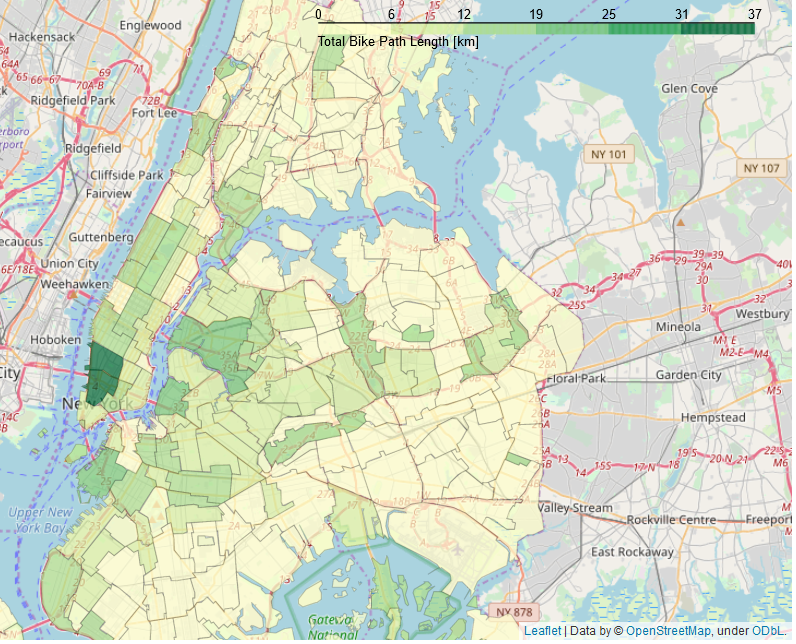
\includegraphics[scale=0.42]{all bike path.png}
    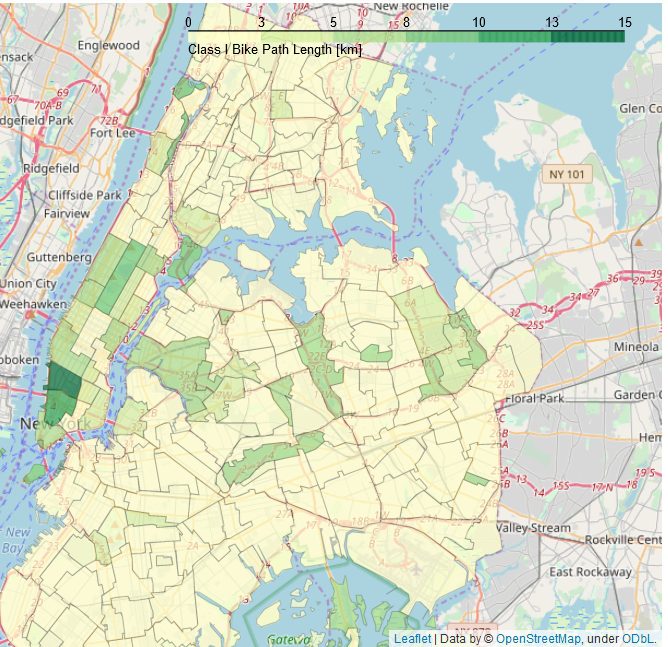
\includegraphics[scale=0.42]{class I bike path.PNG}
    \caption{Left: Total (classes I, II, III) bike path length by NTA area. Right: Class I (grade separated) bike path length by NTA area}
    \label{fig:bikelanes}
\end{figure}


$\bullet$ NYC GeoJSON data: We downloaded GeoJSON data for each of the 195 NTA code areas in NYC. This data was used to make plots in Python using the Folium package. 


\section*{Exploratory Data Analysis}

Upon cleaning and looking at the data for the first time, a clear pattern emerges: the number of rides across all modes of transportation is highly cyclical, with a strong annual seasonality and also a weekly trend. 

For bikeshares, the annual seasonality is most notable, with the number of rides declining sharply during winter months and peaking in July. 

The weekly component shows a marked rise during weekdays, with the peak typically being Wednesday, and a decline during the weekends.

\subsection*{Seasonality}
In our analysis it is prudent to model and perhaps decompose the seasonality component from the data. We assume the data can be decomposed as the following: 
\begin{equation}
    \log{N}_t = n_{baseline} + \delta n_{weekly} + \delta n_{seasonal} +  \epsilon_t,
\end{equation}
where $\log{N}_t$ is the logarithm of the ridership at time $t$; $\delta N_{weekly}, \delta N_{seasonal}$ are the weekly and seasonal components respectively, $N_{baseline}$ is the baseline level, and $\epsilon_t$ is an error term that possibly depends on weather, pricing, the day-to-day variations of the system and any long-term trends.


The first task at hand is to have some estimate of the magnitude of the various cyclical and seasonal effects. To estimate the weekly effect, we simply calculate, over the period of year 2018, the log difference between the ridership of a particular weekday and the annual average ridership. We find a small but highly statistically significant weekly effect: for all other modes, ridership peaks on Wednesdays and fall off earlier and later in the week; the fluctuation is about 10\%; however, Uber behaves differently, with ridership peaking on Fridays. In figure 2, we show the weekly component of the ridership anomaly.

After understanding the weekly component, we move on to the seasonal component of the ridership with the weekly fluctuation removed by subtracting by the mean weekly anomaly. In figure 3, we show the resulting annual seasonality for the year 2018. We see that whereas other modes show somewhat steady ridership during the year, with only noticeable drops during July 4th, Thanksgiving and the Winter Holiday season, bike share shows dramatic seasonal changes in ridership, peaking in the summer months and reaching its nadir at the end of the year. Clearly, the winter months are correlated with lower bikeshare ridership. During these months, what do the bike riders do instead? To investigate this, we must use a more rigorous model, and that is our motivation for selecting the VAR model with exogenous variables.


\begin{figure}[htbp]
    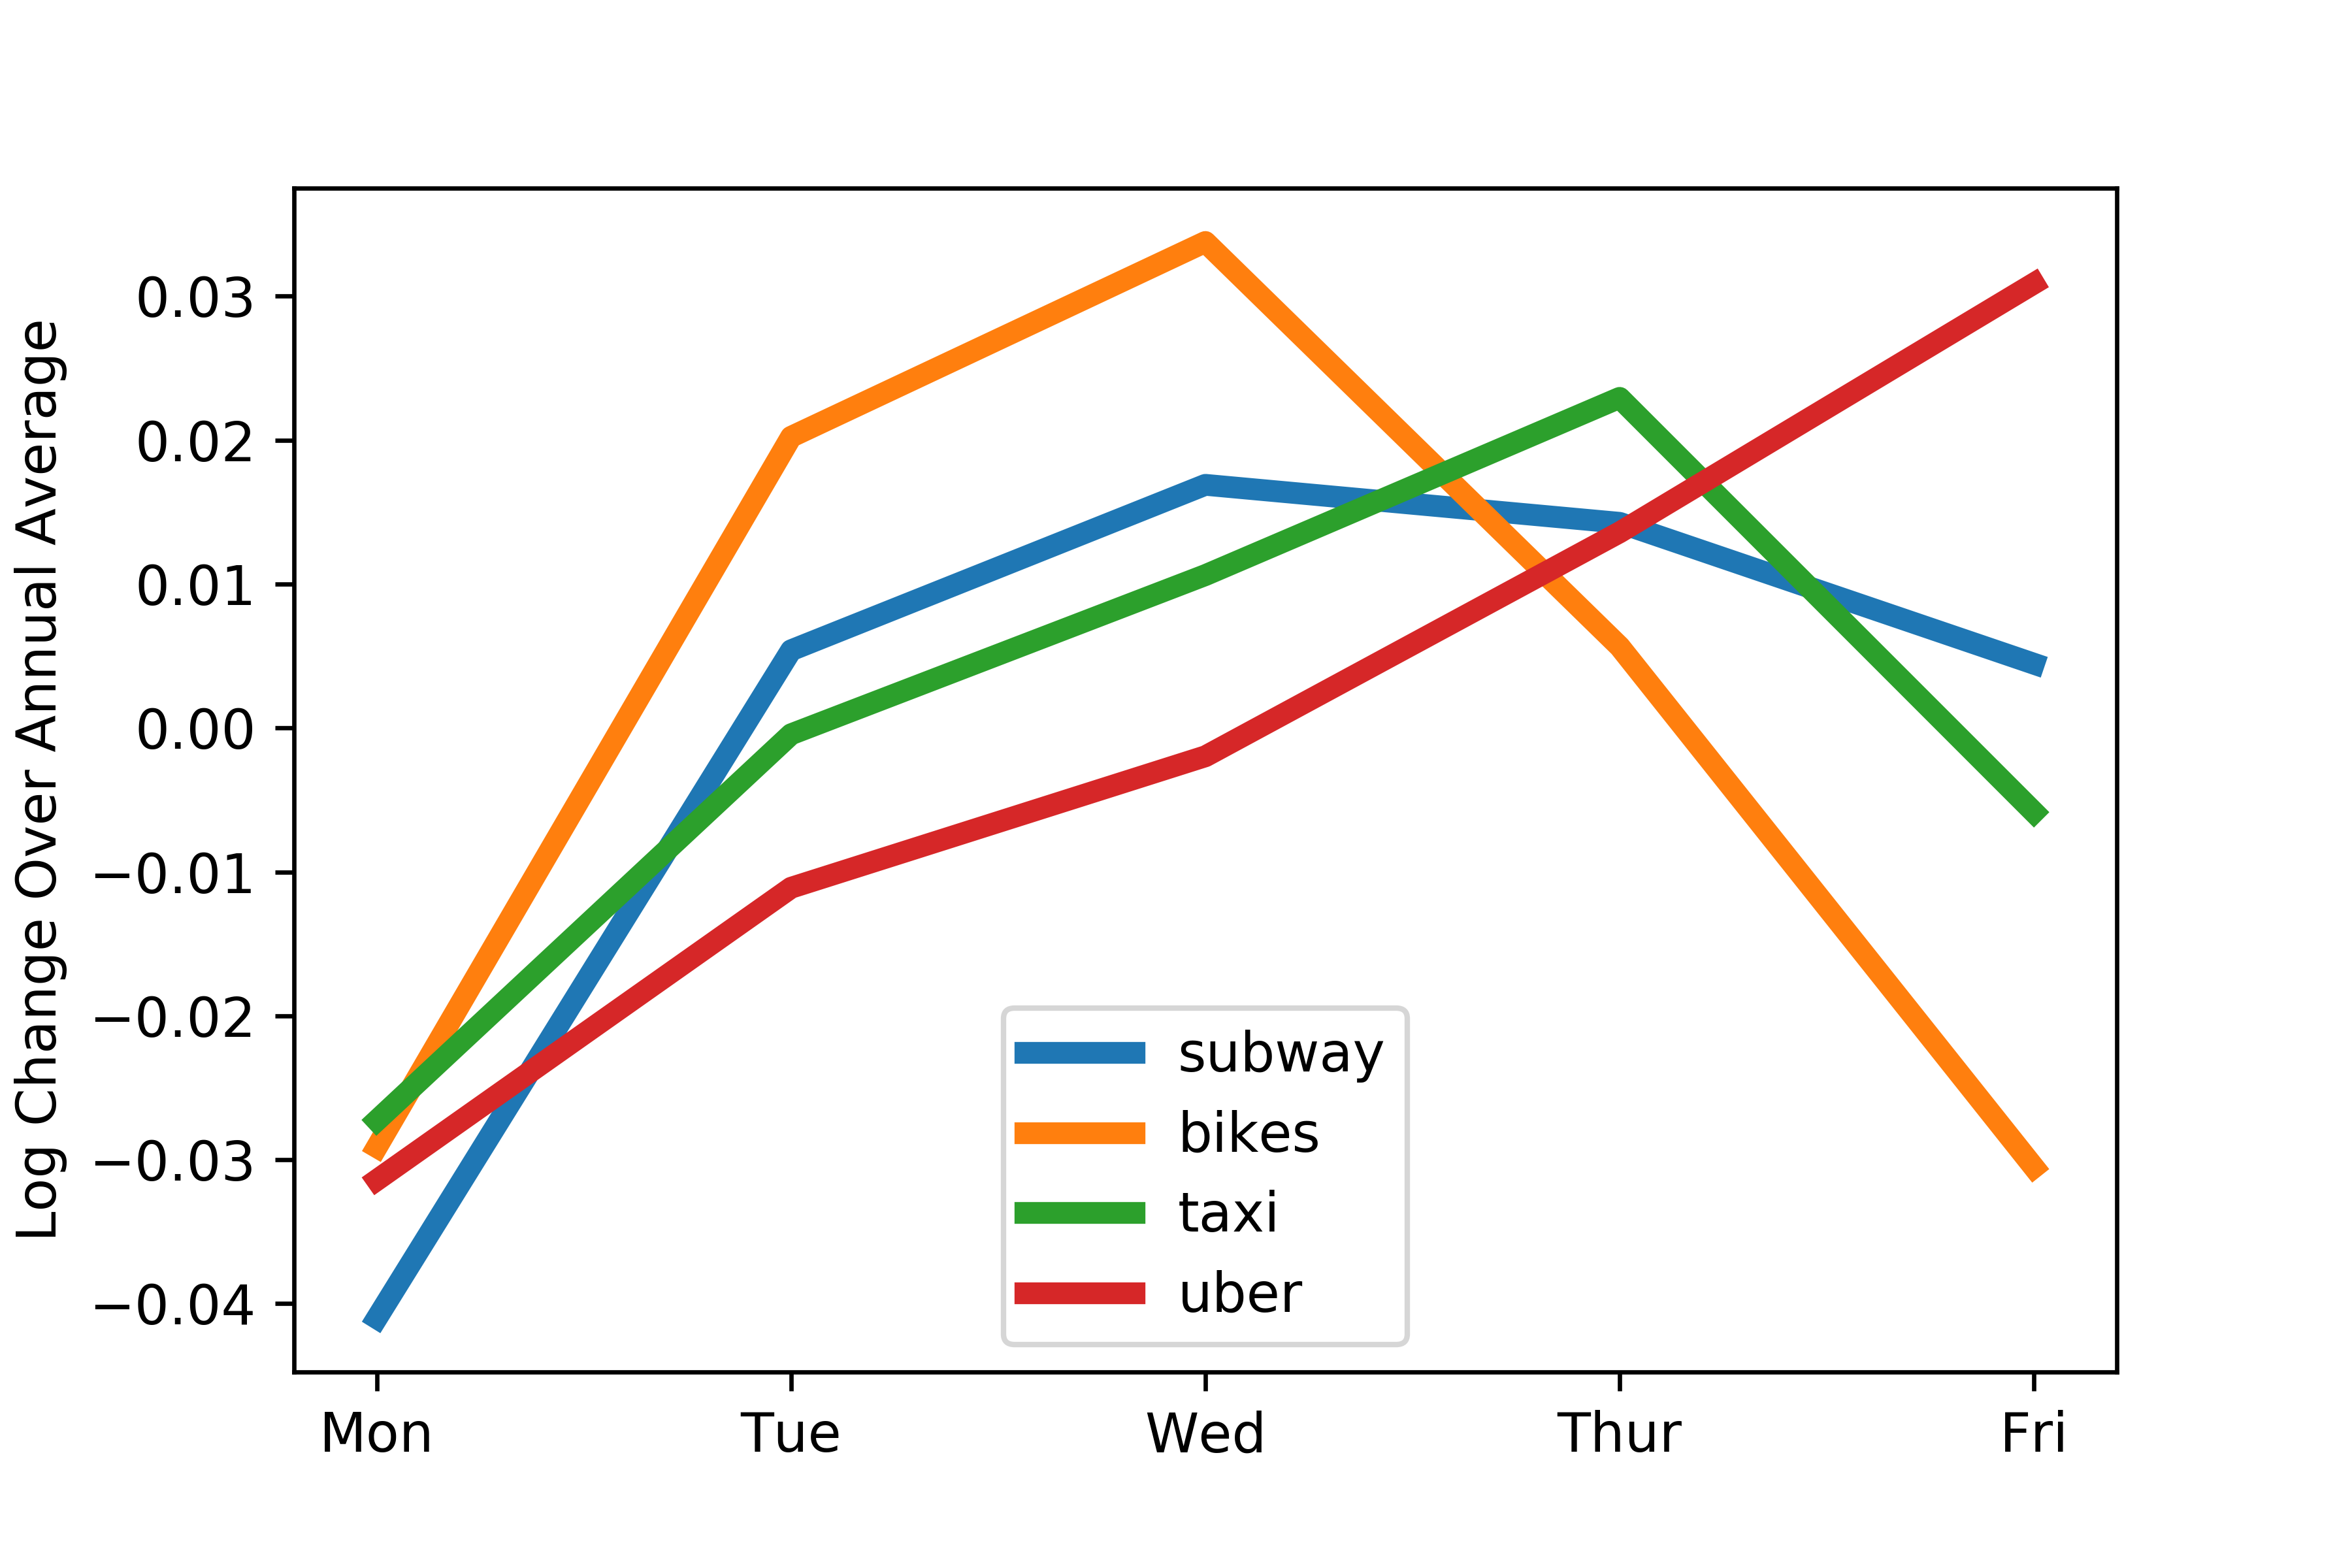
\includegraphics[scale=1.0]{weekly.PNG} \label{fig:weekly}
    \caption{Weekly component of the ridership anomaly}
\end{figure}


\begin{figure}[htbp]
    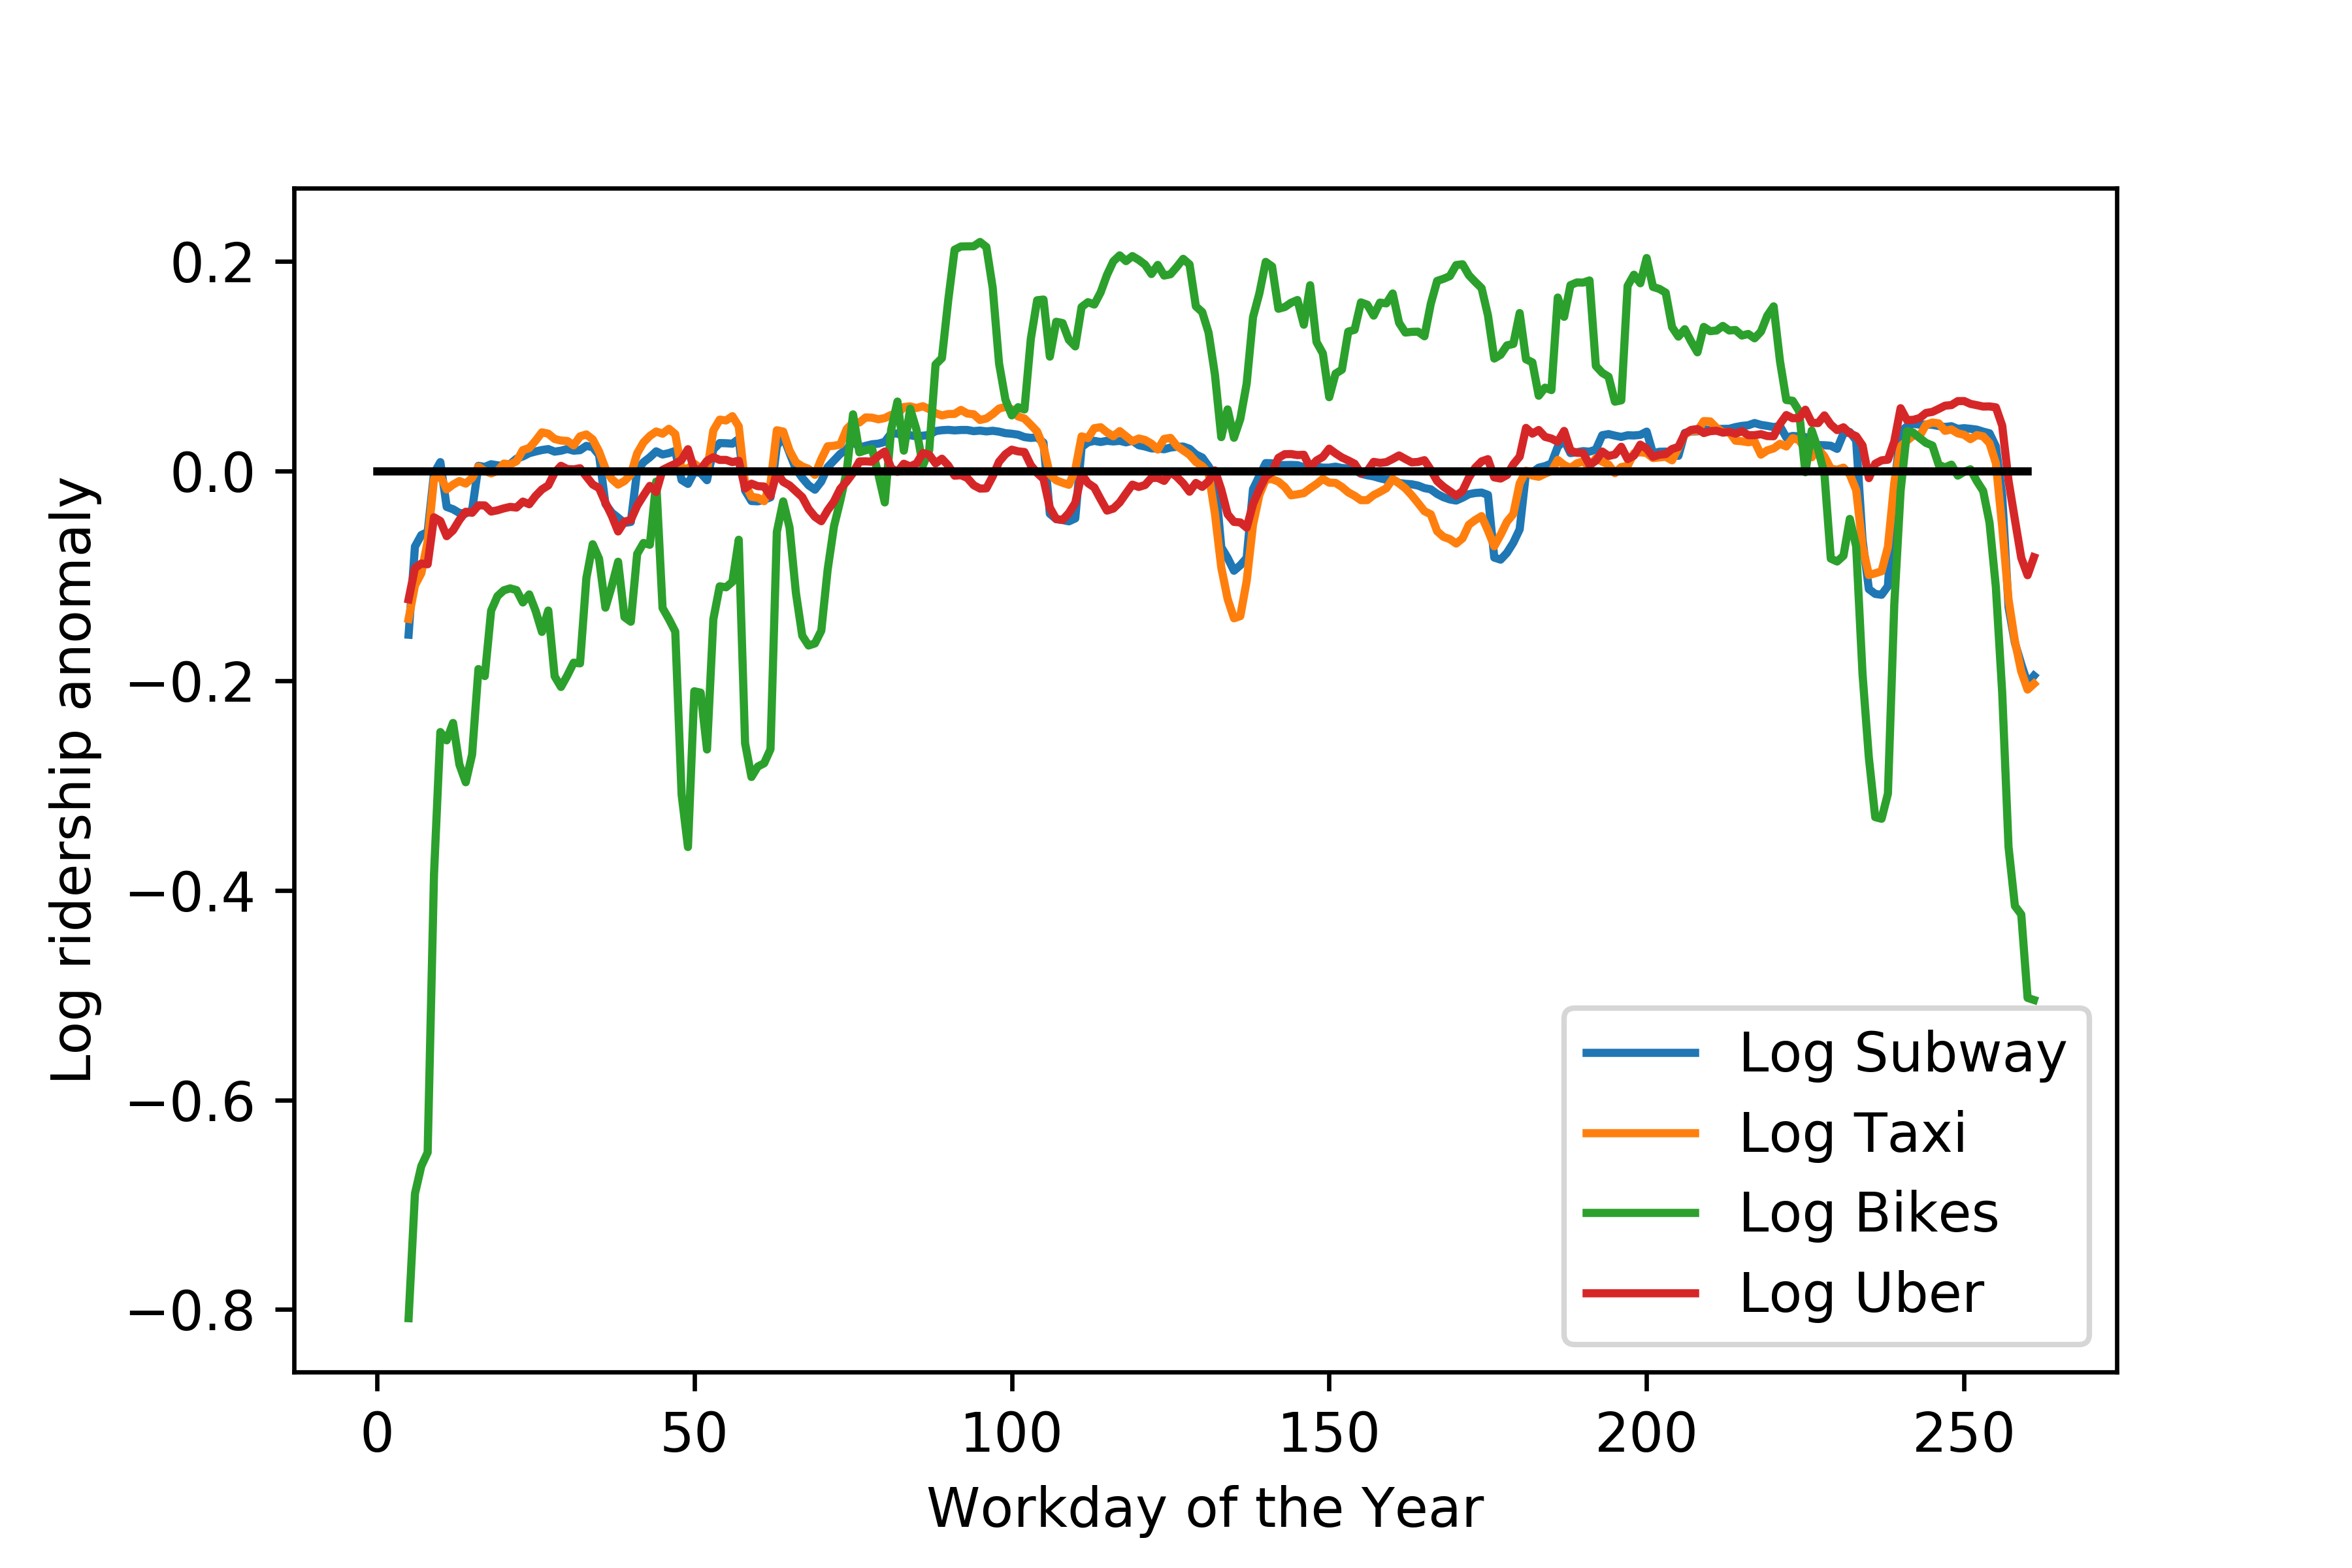
\includegraphics[scale=1.0]{annual.PNG} \label{fig:weekly}
    \caption{Annual component of the ridership anomaly, with weekly component removed}
\end{figure}

To estimate the seasonal effect, we need to apply a filter to mask out the short-term variations and look at the variation on a long timescale. To do this, we first find the monthly averages of ridership, and take its difference in logarithm. Next, we perform a linear spline on this monthly timeseries, and then interpolate between the monthly data-points. This gives us a smooth trend for ridership over a year. This gives us the monthly component of seasonality.

\section*{Visual Analysis using Maps and GIS}

We plot on NYC street map the number of total bike rides (Figure 4)  and shared rides (such as Uber, Lyft, Via, Juno) (Figure 5) in the year of 2017, for each NTA included in the corresponding datasets. We observe obvious spatial heterogeneities in both plots. For instance, Manhattan area has the most bike rides, as well as the most bike lanes. This motivates us to investigate the associations between bike lane lengths, riding patterns, and social-economic factors.


\begin{figure}[htbp]
    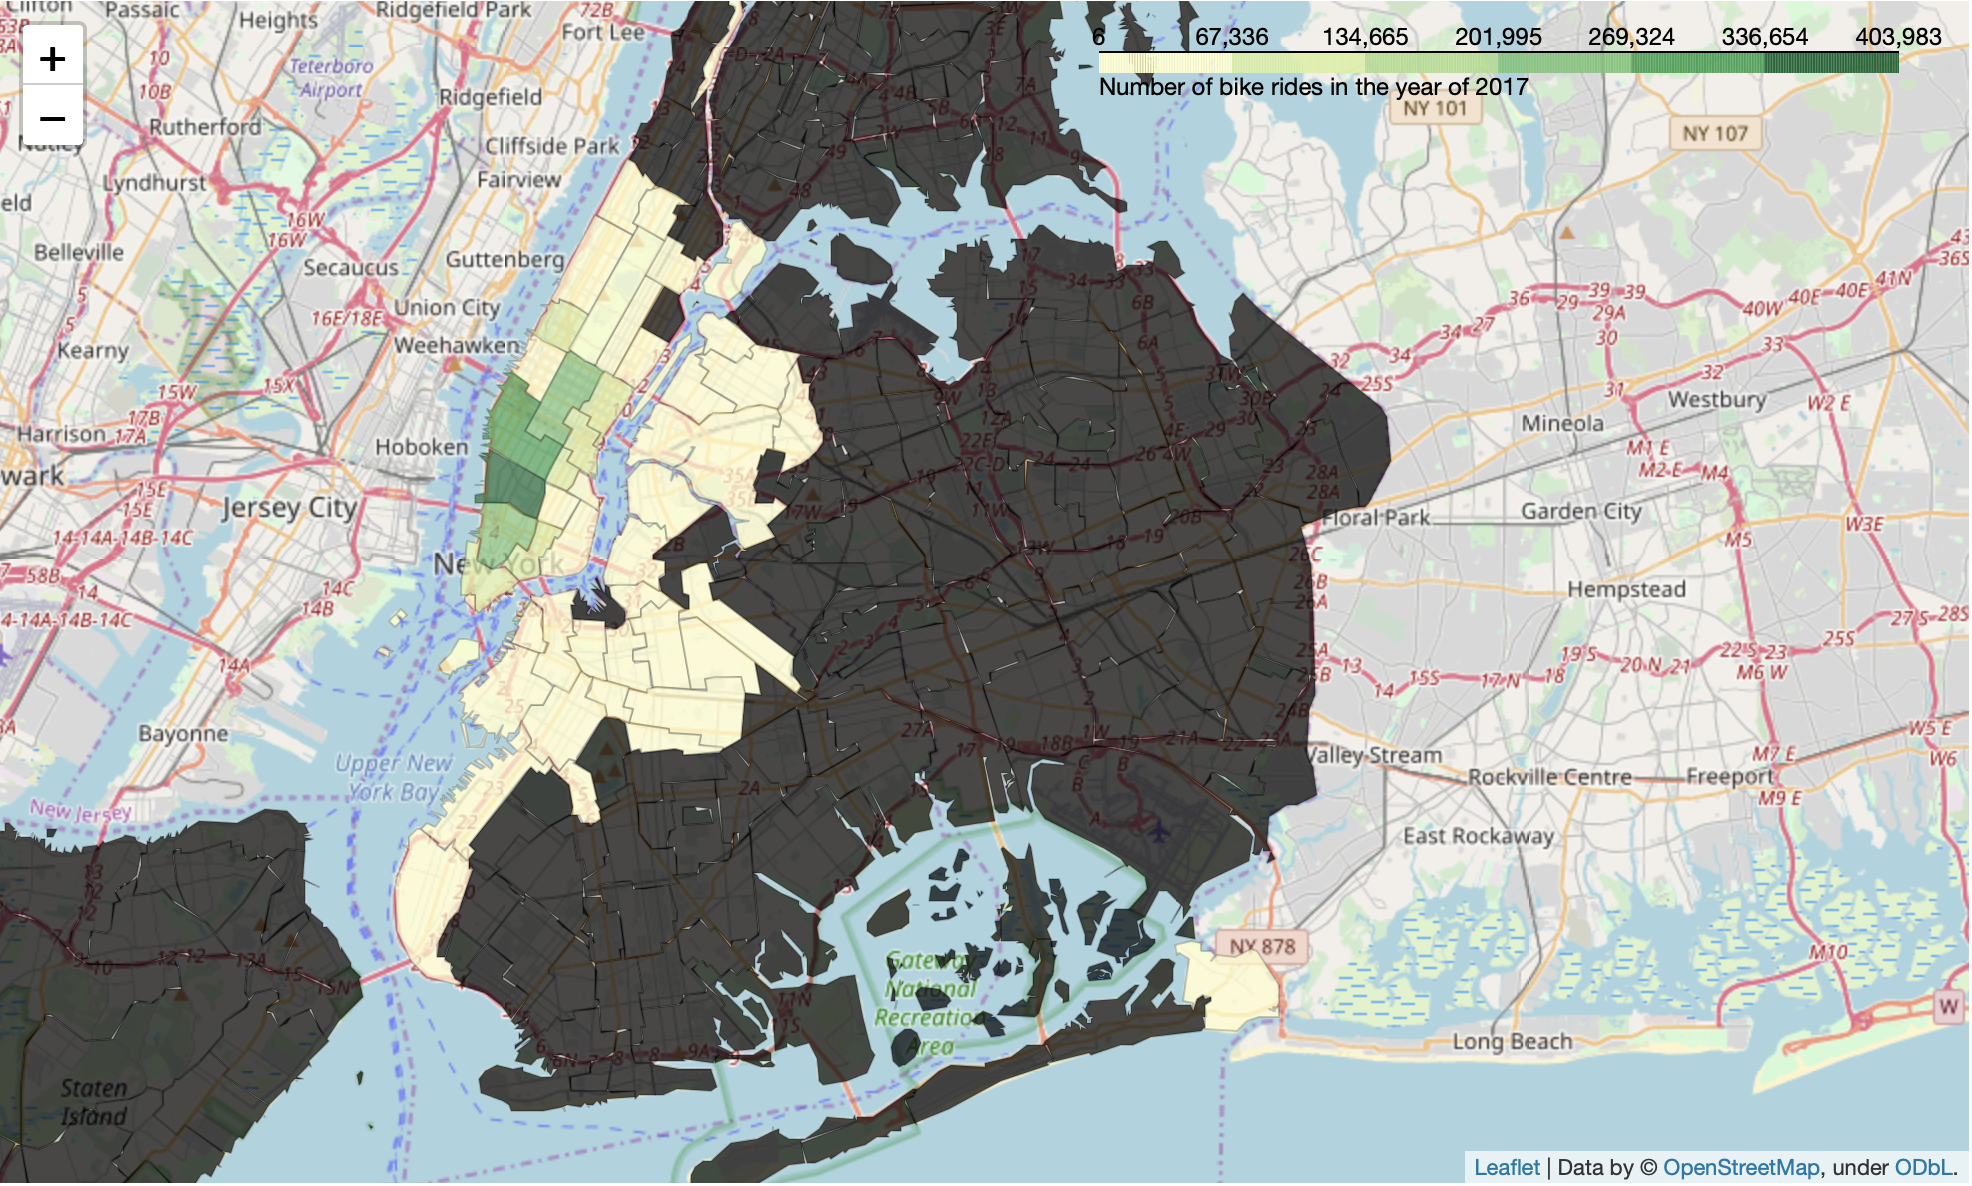
\includegraphics[scale=0.3]{Number_bike_rides_2017.png} \label{fig:bike}
    \caption{Total number of bike rides of NTA areas included in the given datsets, in the year of 2017. Dark areas are those not included in the given datasets.}
\end{figure}



\begin{figure}[htbp]
    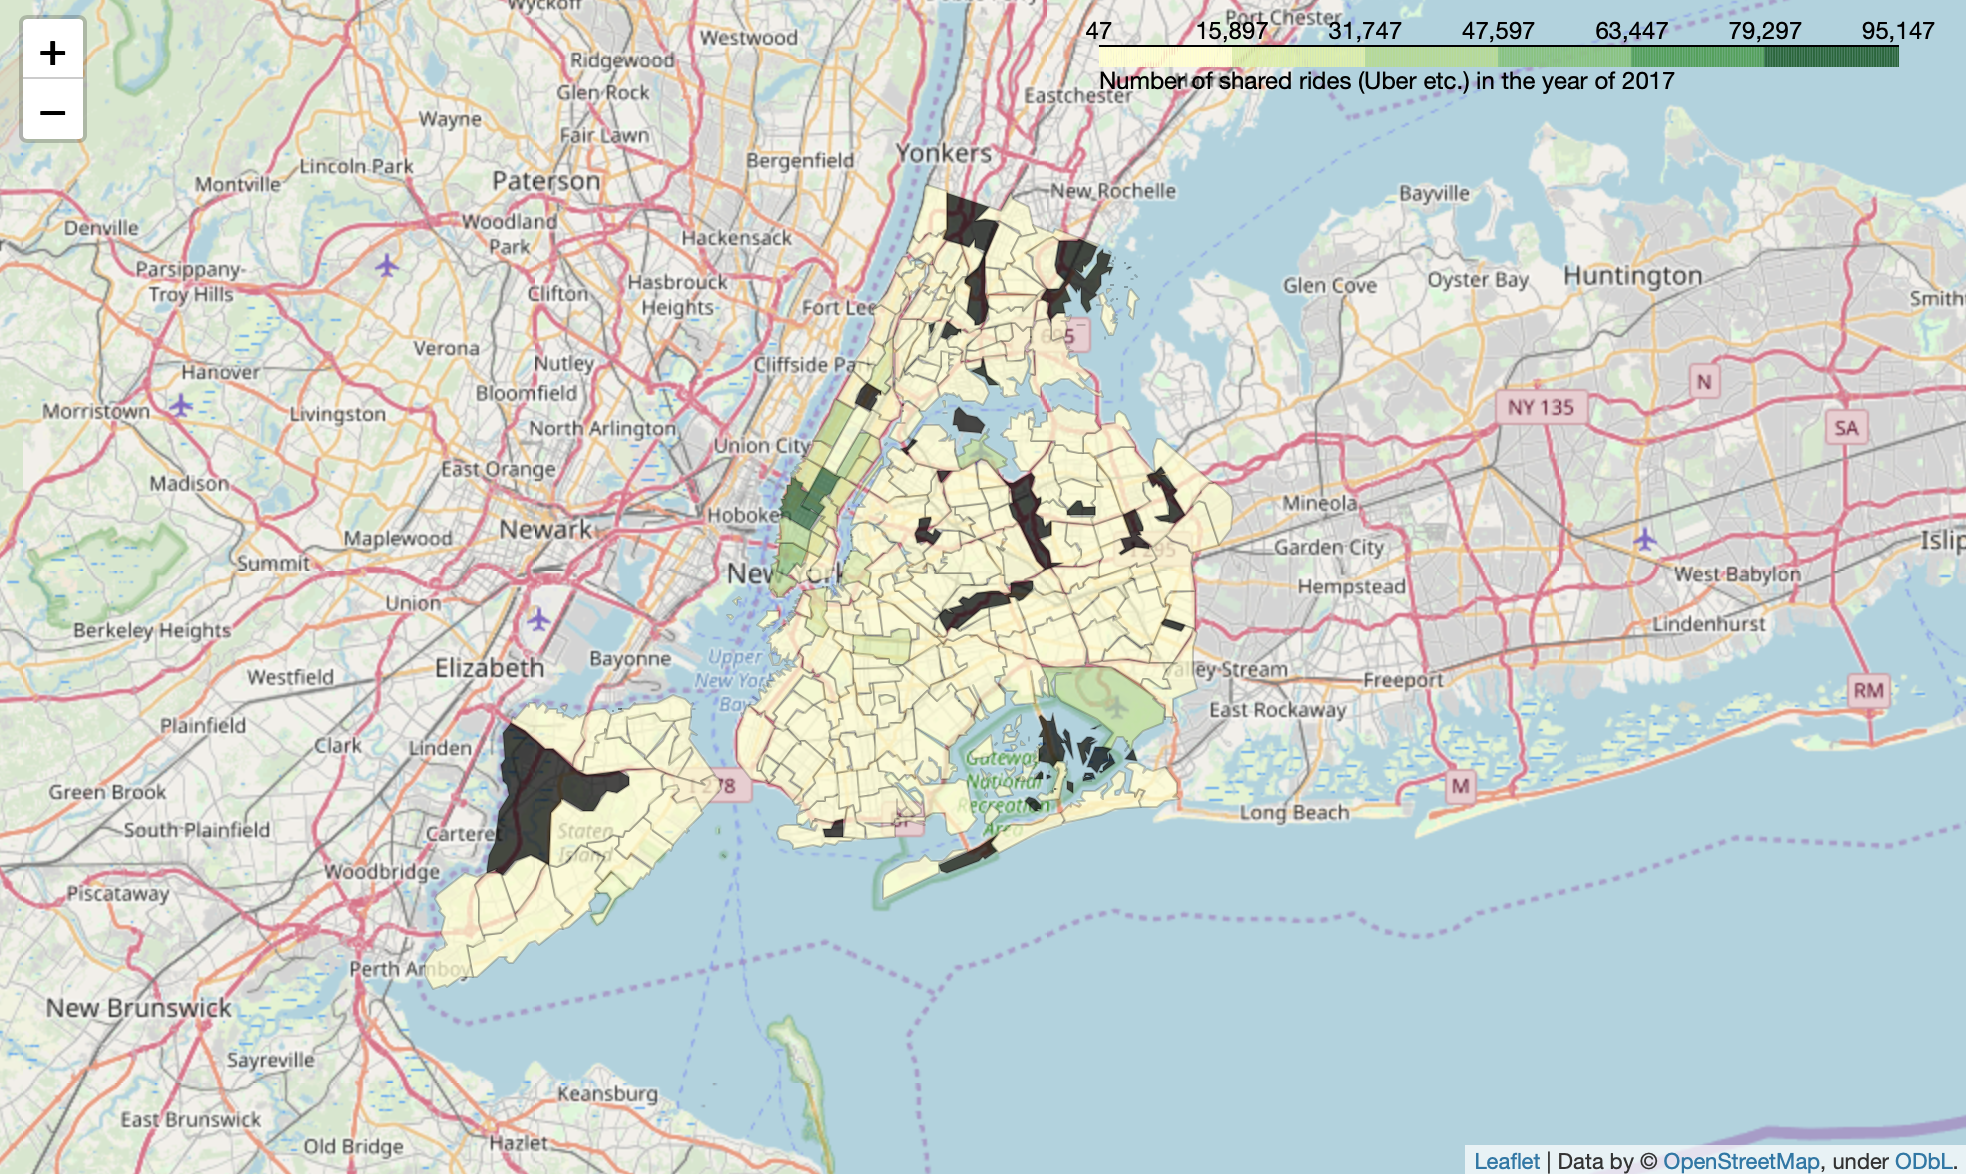
\includegraphics[scale=0.3]{Number_Uber_rides_2017.png} \label{fig:uber}
    \caption{Total number of shared rides (Uber etc.) of NTA areas included in the given datsets, in the year of 2017. Dark areas are those not included in the given datasets.}
\end{figure}



\newpage 
\section*{{\bf Modeling}}



\subsection*{VAR model with Exogeneous Variables}
To study the effect of the interplay of 4 transport modes, we use a Vector auto-regressive (VAR) model to study the changes in ridership in bikes, taxis, subway and uber and lyft. We also include 4 weather variables (temperature anomaly, average wind speed, rain and snow) as exogeneous (independent) variables.

The VAR with exogenous terms is given by
\begin{equation}
    \vec{Y_t} = \mathbf{A_1} \vec{Y_{t-1}} + \mathbf{A_2} \vec{Y_{t-2}} ... + \mathbf{A_l} \vec{Y_{t-l}} + \mathbf{B}\vec{X} + \vec{\epsilon_t},
\end{equation}
where $\vec{Y}_t$ is a vector timeseries, $\mathbf{A}$ are coefficient matrices, $B$ is the matrix of exogeneous variable coefficients, $\vec{X_t}$ are the exogeneous variables at time $t$, $l$ is the lag order, and $\epsilon_t$ is the error term. The results of the VAR model tells us, based on the changes in ridership behavior yesterday, what changes in transport modal composition we expect to see today.

One advantage of VAR is that it allows us to model the response in the system to an impulsive change in one of the endogenous variables. 

There is some debate about the need for stationary when applying VAR models. When the data is non-stationary, i.e. it has a 'unit root' (e.g. long-term trends, cyclic trends or seasonality), the standard errors may be poorly defined. However, others have argued that modelling VAR directly on the quantity of interest, regardless of stationarity, can be more insightful.

In this case, we adopt the cautious approach and use VAR with differencing to make the data stationary. We use the Augmented Dickey-Fuller (ADF) test to test for stationarity. After applying logarithm and differencing once with a shift of 1 (today minus yesterday), we found that all 4 of our endogenous variables had ADF statistics below $10^{-10}$, consistent with stationarity. 

We then apply our VAR model; after trying several lag orders, we found that significance for the coefficients for lag orders $L \ge 3$ were typically insignificant; thus we adopt a VAR(2) model to forecast the behavior of these 4 modes of transport. In the figure below we show the model summary.


\begin{figure}[htbp]
    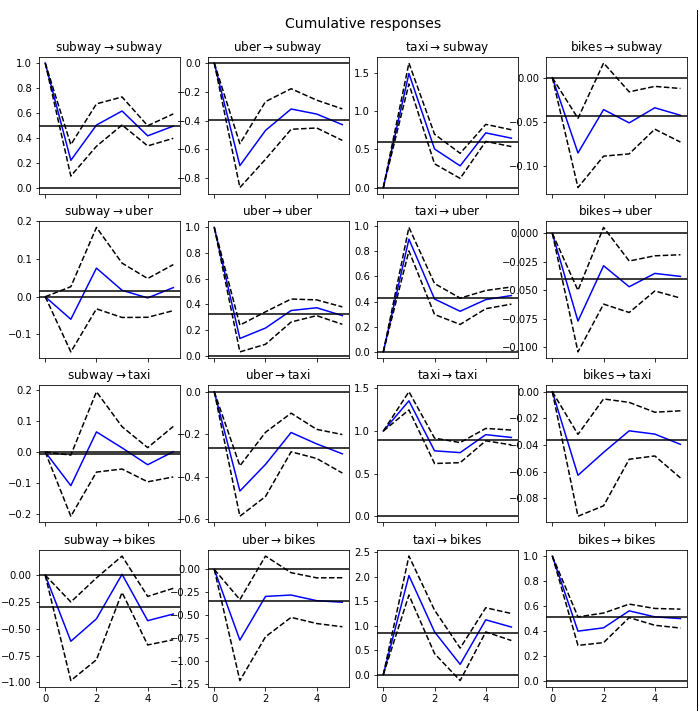
\includegraphics[scale=1.0]{VAR_correlation.PNG} \label{fig:var_matrix}
    \caption{Impulse analysis of our VAR model.}
\end{figure}

We find that, past ridership growth in subway usage and uber and lyft rides tend to reduce future growth in bikeshare usage at statistically significant levels; whereas past ridership growth in taxis is predictive of growth in bikeshare usage.

What are the impact of increased bikeshare ridership on other transport modes? We found that bike usage decreases subway, uber and taxi ridership at statistically significant levels, with the correlation being of roughly equal strength. This shows that bikeshare is essentially replacing other modes of transport when it increases in usage. In other words, when people give up their bikes, they also tend to migrate to taxis, uber and subways in equal proportions.

\subsection*{Weather Effects}
Our VAR model found that the despite the strong seasonal dependence, there is in fact no direct correlation between temperature anomaly, with a $p$-value of $0.9$. Instead, we find statistically significant anti-correlation between bike-share and wind speed, rain and snow, at significance of $1.8, ~3.2, ~4.4 \sigma$ respectively. In other words, for each 1 mph increase in wind speed, the bike ridership decreased by 2\%. For each inch of rain, the ridership decreased by 20\%, and for each inch of snow, the ridership decreased by a whopping 43\%.

In cases of bad weather, which modes saw the most gain? We found that by far, Uber ridership had the most significant correlation between with weather, at above 4-sigma levels. Every inch of rain increased Uber usage by $15\%$, and each inch of snow in fact increased Uber ridership by a whopping $700\%$. 


\begin{figure}[htbp]
    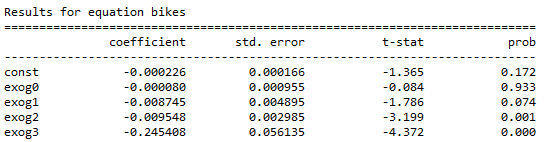
\includegraphics[scale=0.8]{exog.PNG}
    \label{fig:weather_coef}
    \caption{Coefficients of exogenous weather variables effect on bikeshare ridership (log-10 day on day change), exog0, 1, 2, 3 refers to daily temperature anomaly, precipitation (inches), snowfall (inches) and wind (mph) respectively.}
\end{figure}

\begin{figure}[htbp]
    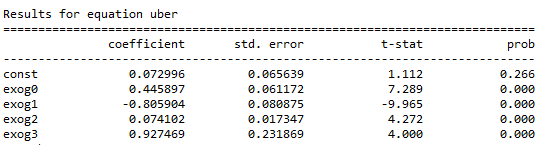
\includegraphics[scale=0.8]{exog_uber.PNG}
    \label{fig:weather_coef_uber}
    \caption{Same as above, except this time the coefficients are for Uber/lyft ridership (log-10 day on day change).}
\end{figure}



\newpage

\subsection*{Linear Regression Model for Spatial Dependence}
Another angle we can explore is the attributes of neighborhoods to better understand what drives people to use bike share. Towards this end, we used linear regression to explore the response variable \textit{rides per population}.
\par In order to account for the impact of seasonality, we aggregated the data for each NTA code for 2017. This leaves a small data set of $\sim45$ NTA areas where citi bike is currently available. After performing feature selection, we find three variables that are significant for the data set at 90\% confidence level (see table below)
\par Number of citi bike stations is the most significant variable, with a coefficient of $0.09$. For an NTA neighborhood of $\sim 50K$, this equates to a $\sim 4.5K$ increase in bike rides (per year). We also see a negative relationship between median age and rides. Unsurprisingly, as people age, it becomes more difficult to take advantage of citi bikes. Therefore, when considering where to add stations, it would be better to focus on areas with younger demographics. We also find that there is no statistically significant dependence between bike lane length and bike share usage, when all other variables are accounted for.
\begin{figure}[htbp]
    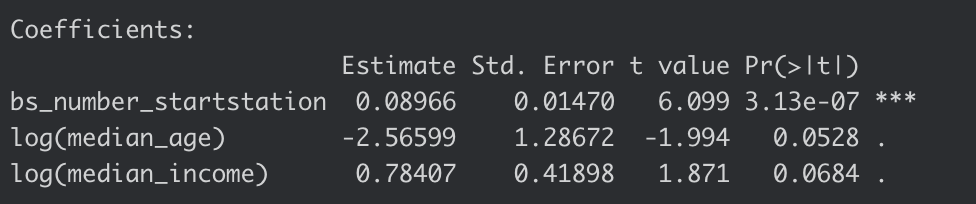
\includegraphics[scale=0.8]{wx.PNG}
    \label{fig:exog}
    \caption{Coefficients of our linear regression analysis}.
\end{figure}


\end{document}
